\subsection{System Engineering \label{sec:sysen}}
Systems engineering is a multidisciplinary approach to the design, implementation and management of complex systems throughout their life cycle (see Figure). It embraces a holistic perspective that takes into account the interactions and interdependencies between different components in order to achieve optimal performance and functionality. Systems engineering deals with work processes, optimisation methods and risk management tools in projects. Systems engineering ensures that all likely aspects of a project or system are considered and integrated as a whole. In the context of the automotive industry, where complex systems and simulations play a central role, the application of systems engineering principles becomes paramount.

\subsubsection{Core Concepts}
    The key principles of systems engineering are as follows:
    \begin{itemize}
      \item Requirements engineering: this phase consists of determining and documenting the needs and constraints that the system must satisfy. In the context of simulation configuration, understanding requirements is crucial to accurately model and simulate real-world automotive scenarios.
      
      \item System design: this phase involves transforming the requirements into a system plan. It involves assigning functions to components, taking into account factors such as efficiency, reliability, and maintainability. For simulation configuration, this step is essential to create a framework that aligns with the specific attributes of automotive simulations.
      
      \item Integration and testing: Systems engineering emphasizes the importance of rigorous testing and integration to ensure that all components work perfectly together. This is particularly relevant in the context of simulation configuration, where the accuracy and reliability of results depend on the effective integration of different simulation parameters.
      
      \item Lifecycle management: Systems engineering goes beyond the initial design and implementation phases. It involves continuous monitoring, maintenance and adaptation to changing requirements throughout the system's lifecycle. This perspective is crucial to the longevity and adaptability of simulation configurations in the dynamic automotive landscape.

    \end{itemize}

    
\subsubsection{V-Model}
The V-model illustrates systems development by highlighting the verification and validation stages. A graphical representation of this model is shown in Figure \ref{fig:v-model}. The system specification and detailed software design are presented on the left-hand side of the “V”, along with the steps leading to implementation. The steps mentioned on the left-hand side must be verified and validated on the right-hand side of the “V”. It also includes the integration of systems and software. Each step on the left is directly linked to a test step. Once the first stage has been successfully completed, the next stage begins.\\

\begin{figure}[H]
    \centering
    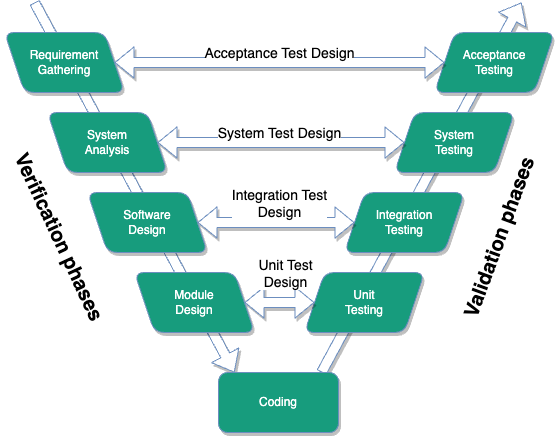
\includegraphics[scale=0.6]{images/V-Model.png}
    \caption{\label{fig:v-model} V-Model }
\end{figure}

With the evolution of technology, many software applications exist to cover these different stages more effectively. 